\documentclass[twoside,openright,titlepage,fleqn,
	headinclude,11pt,a4paper,BCOR5mm,footinclude
	]{scrbook}
%--------------------------------------------------------------
        \newcommand{\myTitle}{Formal methods for systems verification\xspace}
% use the right myDegree option
\newcommand{\myDegree}{Corso di Laurea Magistrale in Informatica\xspace}
%\newcommand{\myDegree}{
	%Corso di Laurea Specialistica in Scienze e Tecnologie 
	%dell'Informazione\xspace}
\newcommand{\myName}{Massimo Nocentini\xspace}
\newcommand{\myProf}{Michele Loreti\xspace}
\newcommand{\myOtherProf}{Mieke Massink\xspace}
\newcommand{\mySupervisor}{Nome Cognome\xspace}
\newcommand{\myFaculty}{
	Facolt\`a di Scienze Matematiche, Fisiche e Naturali\xspace}
\newcommand{\myDepartment}{
	Dipartimento di Sistemi e Informatica\xspace}
\newcommand{\myUni}{\protect{
	Universit\`a degli Studi di Firenze}\xspace}
\newcommand{\myLocation}{Firenze\xspace}
\newcommand{\myTime}{Anno Accademico 2012-2013\xspace}
\newcommand{\myVersion}{Version 0.1\xspace}

%--------------------------------------------------------------
\usepackage[utf8]{inputenc} 
\usepackage[T1]{fontenc} 
\usepackage[square,numbers]{natbib} 
\usepackage[fleqn]{amsmath}  
\usepackage[english]{babel}
\usepackage{ae,aecompl}
\usepackage[pdftex]{graphicx}
\usepackage{latexsym}
\usepackage{amsmath, amsthm, amssymb}
\usepackage{rotating}
\usepackage{boxedminipage}
\usepackage{multicol}

%--------------------------------------------------------------
\usepackage{dia-classicthesis-ldpkg} 
%--------------------------------------------------------------
% Options for classicthesis.sty:
% tocaligned eulerchapternumbers drafting linedheaders 
% listsseparated subfig nochapters beramono eulermath parts 
% minionpro pdfspacing
\usepackage[eulerchapternumbers,subfig,beramono,eulermath,
	parts]{classicthesis}
%--------------------------------------------------------------
\newlength{\abcd} % for ab..z string length calculation
% how all the floats will be aligned
\newcommand{\myfloatalign}{\centering} 
\setlength{\extrarowheight}{3pt} % increase table row height
\captionsetup{format=hang,font=small}
%--------------------------------------------------------------
% Layout setting
%--------------------------------------------------------------
\usepackage{geometry}
\geometry{
	a4paper,
	ignoremp,
	bindingoffset = 1cm, 
	textwidth     = 13.5cm,
	textheight    = 21.5cm,
	lmargin       = 3.5cm, % left margin
	tmargin       = 4cm    % top margin 
}
%--------------------------------------------------------------

\usepackage{hyperref}
\usepackage{listings}
\usepackage{pdfpages}
% My Theorem
\newtheorem{oss}{Observation}[section]
\newtheorem{exercise}{Exercise}[section]
\newtheorem{thm}{Theorem}[section]
\newtheorem{cor}[thm]{Corollary}

\newtheorem{lem}[thm]{Lemma}

\newcommand{\vect}[1]{\boldsymbol{#1}}

% questo comando e' relativo alle correzioni che puo
% apportare il prof se lo desidera.
\newcommand{\prof}[1]{\boldsymbol{#1}}

% instead of boldsymbol I can use the arrow above the letter with
%\newcommand{\vect}[1]{\vec{#1}}

% page settings
% \pagestyle{headings}
%--------------------------------------------------------------
\begin{document}
\frenchspacing
\raggedbottom
\pagenumbering{roman}
\pagestyle{plain}
%--------------------------------------------------------------
% Frontmatter
%--------------------------------------------------------------
%--------------------------------------------------------------
% titlepage.tex (use thesis.tex as main file)
%--------------------------------------------------------------
\begin{titlepage}
	\begin{center}
   	\large
      \hfill
      \vfill
      \begingroup
			\spacedallcaps{\myUni} \\ 
			\myFaculty \\
			\myDegree \\ 
			\vspace{0.5cm}
         
\includegraphics[scale=.065]{logo/unifi}\\
         \vspace{0.5cm}    
         %% -------put here the type of document---ie: Tesi di Laurea
         Elaborato d'Esame
      \endgroup 
      \vfill 
      \begingroup
      	\color{Maroon}\spacedallcaps{\myTitle} \\ \bigskip
      \endgroup
      \spacedlowsmallcaps{\myName}
      \vfill  
      Professori: \itshape{\myProf}, \itshape{\myOtherProf}
      \vfill  
      \myTime
      \vfill                      
	\end{center}        
\end{titlepage}   
%--------------------------------------------------------------
% back titlepage
%--------------------------------------------------------------
   \newpage
	\thispagestyle{empty}
	\hfill
	\vfill
	\noindent\myName: 
	\textit{\myTitle,} 
	\myDegree, \textcopyright\ \myTime
%--------------------------------------------------------------
% back titlepage end
%--------------------------------------------------------------
\pagestyle{scrheadings}
%--------------------------------------------------------------
% Mainmatter
%--------------------------------------------------------------
\pagenumbering{arabic}

% settings for the lstlisting environment
\lstset{
	language = R
	, numbers = left 
	, basicstyle=\sffamily%\footnotesize
%	, frame=single
	, tabsize=2
	, captionpos=b
	, breaklines=true
	, showspaces=false
	, showstringspaces=false
}

\tableofcontents

\newpage

\section*{Goal}
This document collects my work on the course \emph{Formal methods for
  system verification}.

\subsection*{Some useful web location}
The source of the exercises is:\\
\href{http://www-i2.informatik.rwth-aachen.de/i2/mvps11/}{
  http://www-i2.informatik.rwth-aachen.de/i2/mvps11/}
\\\\
This document is hosted in the following \texttt{git} repository:
\\
\href{https://github.com/massimo-nocentini/metodi-formali-verifica-sistemi}{
  https://github.com/massimo-nocentini/metodi-formali-verifica-sistemi}


\newpage

\section*{Licences}

\subsection*{Text contents}
All the text content is distributed under:\\
\textbf{ This work is licensed under the Creative Commons Attribution,
  NonCommercial, ShareAlike 3.0 Unported License. To view a
  copy of this license, visit\\
  \href{http://creativecommons.org/licenses/by-nc-sa/3.0/}{http://creativecommons.org/licenses/by-nc-sa/3.0/}\\
  or send a letter to Creative Commons, 444 Castro Street, Suite 900,
  Mountain View, California, 94041, USA.}

\begin{center}

\includegraphics{cc-icons-eps/by}

\includegraphics{cc-icons-eps/cc}

\includegraphics{cc-icons-eps/nc}

\includegraphics{cc-icons-eps/sa}
\end{center}

\subsection*{Sources}
All sources are distributed under, where the word ``Software'' is
referred to all of the sources that are present in this work: \\
\textbf{
  Copyright (c) 2011 Massimo Nocentini\\
  Permission is hereby granted, free of charge, to any person
  obtaining a copy of this software and associated documentation files
  (the "Software"), to deal in the Software without restriction,
  including without limitation the rights to use, copy, modify, merge,
  publish, distribute, sublicense, and/or sell copies of the Software,
  and to permit persons to whom the Software is furnished
  to do so, subject to the following conditions:\\
  The above copyright notice and this permission notice shall be
  included in all
  copies or substantial portions of the Software.\\
  THE SOFTWARE IS PROVIDED "AS IS", WITHOUT WARRANTY OF ANY KIND,
  EXPRESS OR IMPLIED, INCLUDING BUT NOT LIMITED TO THE WARRANTIES OF
  MERCHANTABILITY, FITNESS FOR A PARTICULAR PURPOSE AND
  NONINFRINGEMENT. IN NO EVENT SHALL THE AUTHORS OR COPYRIGHT HOLDERS
  BE LIABLE FOR ANY CLAIM, DAMAGES OR OTHER LIABILITY, WHETHER IN AN
  ACTION OF CONTRACT, TORT OR OTHERWISE, ARISING FROM, OUT OF OR IN
  CONNECTION WITH THE SOFTWARE OR THE USE OR OTHER DEALINGS IN THE
  SOFTWARE.  }


\chapter{Quantitative Part}



\section{Basic Definitions}

In this section we recall basic definitions used in the remaing part
of the \emph{qualitative project} paper.

\subsection{Stochastic Processes}

A \emph{stochastic process} $p$ is a $\mathcal{T}$-indexed family of
random variables $X_i$, formally $p = \{X_i: i \in \mathcal{T}\}$, in
particular $p$ is called \emph{discrete} if $\mathcal{T} = \mathbb{N}
$, otherwise $p$ is called \emph{continuous} if $\mathcal{T} =
\mathbb{R} $.


\subsection{Discrete Time Markov Chains}

A \emph{Discrete Time Markov Chain} (DTMC) is a discrete stochastic
process such that, given $\Omega$ a sample space, $X_i:\Omega
\rightarrow \mathbb{N}, \forall i\in \mathbb{N} $.
% Usually a DTMC is
% modeled with a tuple $(S, P, AP, L)$ such that:
% \begin{itemize}
% \item $S$ is a finite set of \emph{states};
% \item $P$ is a function such that $P:S\times S \rightarrow [0,1]$,
%   where $\sum_{v \in S}{P(s,v)} = 1, \forall s \in S $;
% \item $AP$ is a set of \emph{atomic propositions};
% \item $L$ is a function such that $L:S \rightarrow AP$.
% \end{itemize}

\section{Herman's Stabilization algorithm}

This paper study an algorithm about self-stabilization of
fault-tolerant systems in a distributed environment. We can abstract a
fault-tolerant system with a network of processes and the goal is to
build a protocol which, applied to an initial configuration $i$ of the
network, produces a new configuration $c$ such that:
\begin{itemize}
\item $c$ satisfies some property of interest;
\item the protocol requires a \emph{finite} number of steps to produce
  $c$;
\item there is no intervention of outside objects in order to produce
  $c$.
\end{itemize}
In the following section we state formally the problem described above
and the Herman algorithm under study. We've used the article \cite{
  KNP12a} to make our formalizations.

\subsection{Background}

Herman protocol \cite{Her90} is applied to a network of processes
$p_i$ where $i \in \{1,\ldots, n\}$, structured in an oriented ring
and ordered anticlockwise. This protocol is synchronous, that is
actions taken by each process $p_i$ happen simultaneously, no
interleaving are present. Following the presentation given by Herman,
it is possible to represent each process $p_i$ with a single
\emph{bit} $x_i$ and the entire network with a DTMC. With those basics
we're ready to introduce some concepts that we want to study with a
simulation using PRISM \cite{KNP11}.

We define a \emph{network configuration} as a state of the DTMC with
$n$ processes, so a tuple $(x_n, \ldots, x_1) \in \{0,1\}^n$. In the
ring may exist one or more processes that have \emph{tokens} and those
can be passed between processes $p_i$ and $p_{i+1}$ (so always to the
right neighbor). A process $p_i$ has a token if $x_i =
x_{i-1}$. Finally, a network configuration is \emph{stable} if
$\exists! p_i$ that has a token.
\\\\
From the above definitions follow these facts:
\begin{itemize}
\item given a network with $n$ processes, the set of states $S$ of the
  underlying DTMC has cardinality $2^n$. This can be proved saying
  that each state $s\in S$ has $n$ components, each component has $2$
  possible value, hence $|S| = 2^n$;
\end{itemize}

\subsection{Protocol rule}

Let $k$ be a generic execution step, the protocol consists of the
following rule:
\begin{displaymath}
  \begin{split}
    x_{i}^{(k+1)} &:= x_{i-1}^{(k)} \quad &\text{if } x_{i}^{(k)} \not=
    x_{i-1}^{(k)}\\
    x_{i}^{(k+1)} &:= random(0,1) \quad &\text{if } x_{i}^{(k)} =
    x_{i-1}^{(k)}
  \end{split}
\end{displaymath}
where $x_{i}^{(k)}$ is the value of $x_i$ at step $k$, $:=$ means
assignment and $random$ is a function that simulate a unbiased coin
toss. In \autoref{table:herman-protocol-execution-example} we report a
simple example of protocol execution applied to 5 processes, starting
from the network configuration $(1, 1, 0, 0, 1)$.
\begin{table}[ht]
  \begin{center}
    \begin{tabular}{cccc}
      \hline
      step & $(x_5, x_4, x_3, x_2, x_1)$ & Tokens owners & coin tosses \\ 
      \hline     
      1 & $(1, 1, 0, 0, 1)$ & $p_5, p_3, p_1$ & $x_1^{(2)}:= 0,
      x_3^{(2)}:= 1, x_5^{(2)}:= 1$  \\
      2 & $(1, 0, 1, 1, 0)$ & $p_3$ & $x_3^{(3)}:= 0$  \\
      3 & $(0, 1, 0, 0, 1)$ & $p_3$ & $x_3^{(4)}:= 0$  \\
      4 & $(1, 0, 0, 1, 0)$ & $p_4$ & $x_4^{(5)}:= 0$  \\
      5 & $(0, 0, 1, 0, 1)$ & $p_5$ & $\ldots$  \\ 
      \hline
    \end{tabular}
    \caption{Example of protocol execution}
    \label{table:herman-protocol-execution-example}
  \end{center}
\end{table}

It is interesting to observe these facts:
\begin{itemize}
\item from network configurations $\forall i:x_i=0$ and $\forall
  i:x_i=1$ of length $n$, it is possible to reach every other state by
  applying the second case of the protocol rule;
\item the protocol doesn't stop when a stable network configuration is
  reached. In fact, in a stable configuration, let $p_i$ be the token
  owner: depending its coin tossing, $p_i$ can decide to pass the
  token to $p_{i+1}$ or to keep it another turn (in the example
  reported above, if at step 4 would have been $x_4^{(5)}:= 1$ the
  next configuration would have been $(0, 1, 1, 0, 1)$, with $p_4$
  token owner again);
\item in order to have an estimate number of steps necessary to reach
  a stable configuration we do a PRISM simulation, using the
  \emph{Confidence Interval} method, with 1000 samples. Looking at the
  log:
\begin{verbatim}
Path length statistics: average 5.4, min 1, max 29
\end{verbatim}
  So the average number of necessary steps for reaching a stable
  configuration is $5.4$.
\end{itemize}

\subsection{Interesting properties}

In this section we verify if Herman protocol satisfy some desired
properties, in particular if a stable configuration is eventually
reached and if it is reached within $k$ steps.

Before get deep into properties verification it is important to
understand that if we'd have used a \emph{qualitative} model checker
to verify if a stable configuration is \emph{always} eventually
reached, the result would be \emph{reject}. To see why, let the DTMC
be in the state $(1,1,1,1,\ldots,1,1)$ and, repeating the application
of rule two of the protocol, for all $p_i$ the toin coss results in
$1$, getting $(1,1,1,1,\ldots,1,1)$ again. There exists an infinite
path on the DTMC which catch the previous behavior, hence that path is
the counterexample for ``from the initial state
$(1,1,1,1,\ldots,1,1)$, is a stable configuration \emph{always}
eventually reached?''
\\\\
The followings are properties we want to check:
\lstinputlisting{quantitative-project/herman7.pctl}
The results are respectively: $true, false, true, 0.8757, 5.4933$.



% \chapter{Some exercises}
% 
\section{Series 1}
\subsection{Exercise 1}
\subsubsection{Question a}
The set $\mathcal{F}$ is built according the following rules, $\forall
A \subseteq \Omega$, with $\Omega$ a countably infinite set:
\begin{enumerate}
\item $|A| < \infty \rightarrow A \in \mathcal{F}$
\item $A \in \mathcal{F} \rightarrow A^c \in \mathcal{F}$
\end{enumerate}
\begin{proof}
  We try to make some attempt to study the minimal composition of
  $\mathcal{F}$, induced by its definition.

  By rule 1, $\emptyset \in \mathcal{F}$ holds because $|\emptyset| <
  \infty$. By rule 2 follow $\Omega \in \mathcal{F}$, because
  $\emptyset \in \mathcal{F}$ and $\Omega = \emptyset^c$. So far we
  have $\mathcal{F} = \{\emptyset, \Omega \}$. Using rule 1 again,
  every finite set $A \subset \Omega$ belong to $\mathcal{F}$, hence
  $\mathcal{F} = \{\emptyset, \Omega \} \cup \{A \subset \Omega:
  |A|<\infty\}$. But the sets we added in the last step in
  $\mathcal{F}$ allow us to apply rule 2 on each of them, forcing to
  add the complement of each: $\mathcal{F} = \{\emptyset, \Omega \}
  \cup \{A \subset \Omega: |A|<\infty\} \cup \{A^c \subset \Omega:
  |A|<\infty\}$ (note that the set $A^c$ is infinite where $A$ is
  finite and $\Omega$ is coutably infinite).

  The definition of $\mathcal{F}$ doesn't allow to add any other sets,
  hence we stop here in its construction.

  To show that $\mathcal{F}$ is not trivial, we have to show that
  exists a set which is in $2^{\Omega}$ but not in $\mathcal{F}$. In
  order to find such set, we have to exclude any finite set because by
  definition and the argument described above, it belong to
  $\mathcal{F}$. Hence it must be an infinite set. But we cannot
  choose an infinite set which is the complement of a finite one,
  otherwise it is in $\mathcal{F}$ too. Hence the choice restrict to
  an infinite set $A$ such that both $A$ both $A^c$ (which is infinite
  too, otherwise $A \in \mathcal{F}$ by rule 1) are not in
  $\mathcal{F}$. The set that contains every pair of sets $A$ and
  $A^c$, both infinite, is $2^\Omega$ and this finish the proof.
\end{proof}
To make an example choose $\Omega = \mathbb{N}, A = \{2i:i \in
\mathbb{N}\}$.

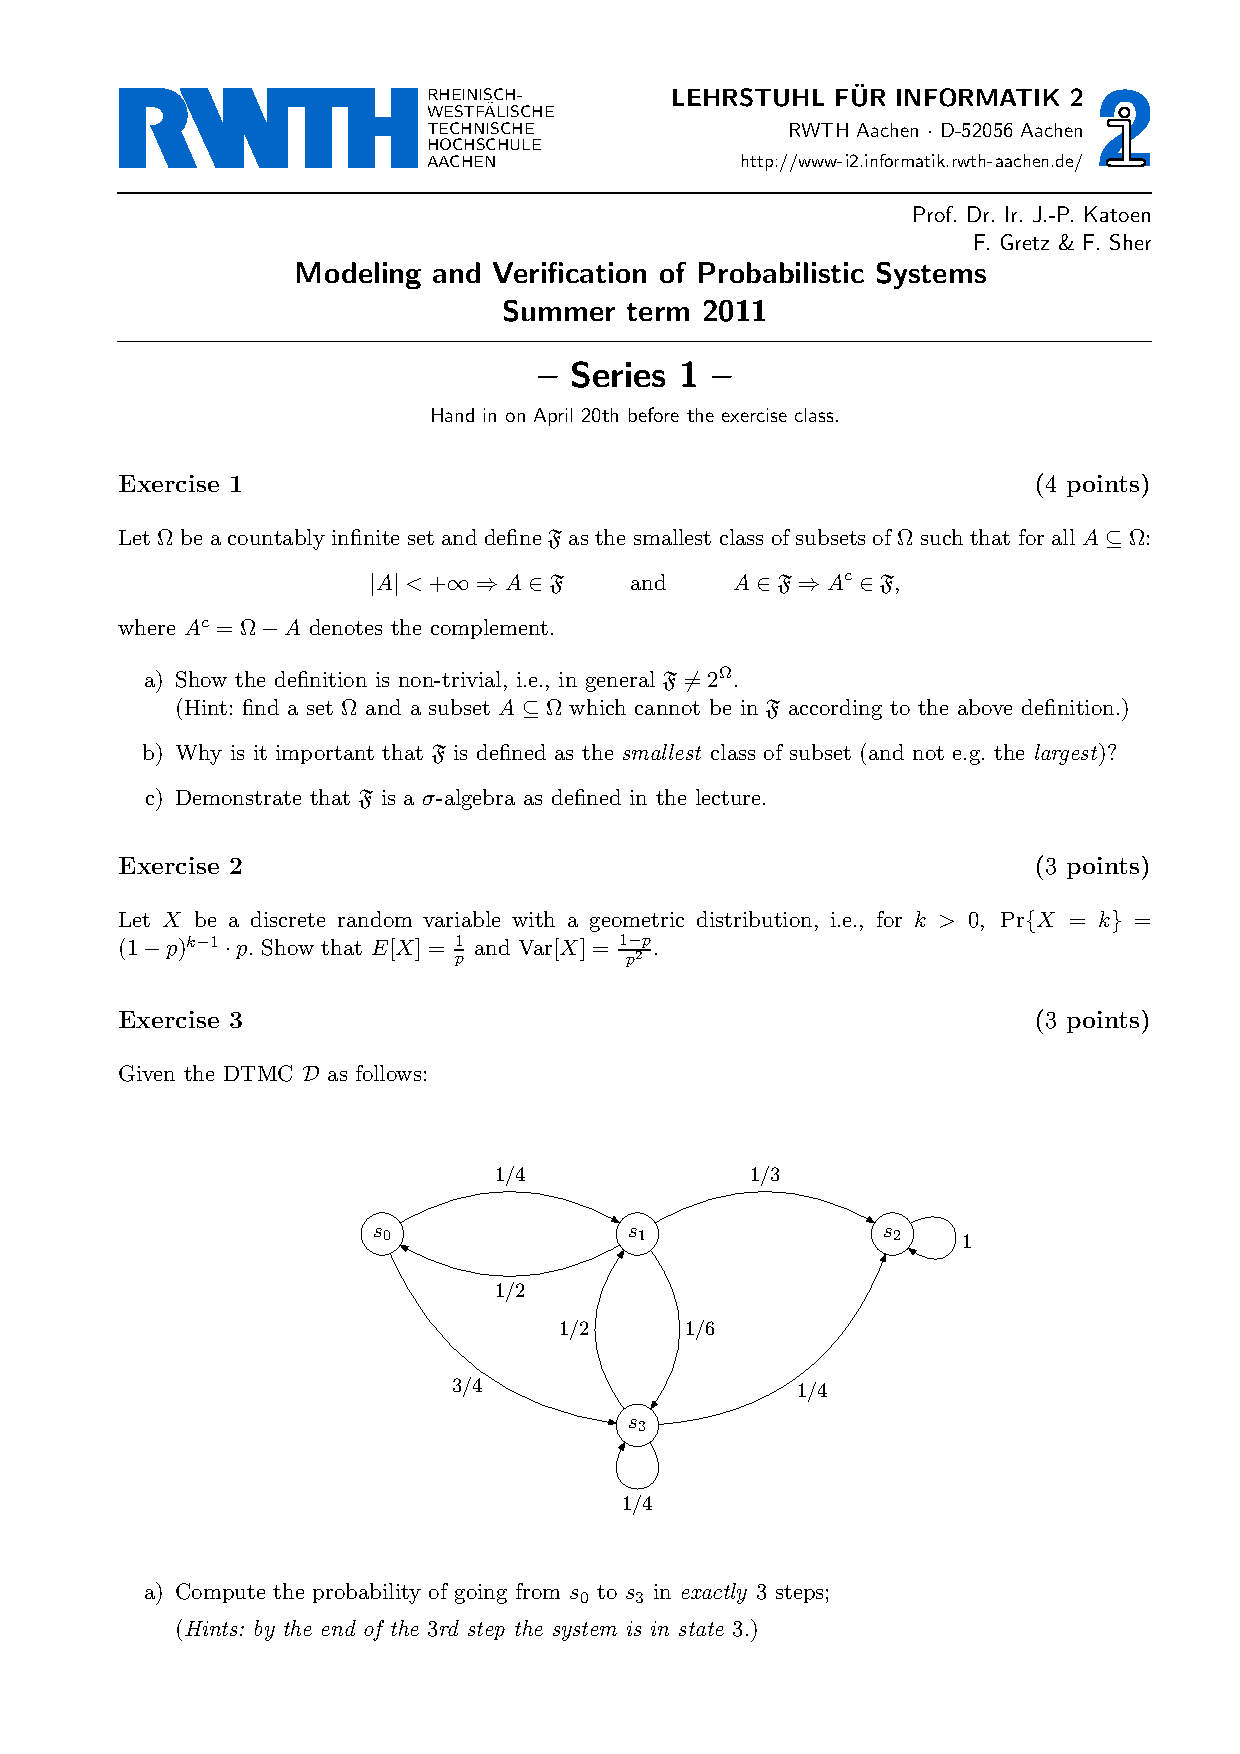
\includepdf[pages={-}]{pdf-to-include/sheet01.pdf}

\subsubsection{Question b}
It is important that $\mathcal{F}$ is defined as the \emph{smallest}
class of subset because the constraint ``smallest'' allow our building
process to stop where we mention before, that is, it allow to not
include pairs of sets $A$ and $A^c$ both infinite. This is the main
difference between $\mathcal{F}$ and $2^\Omega$, having a non trivial
set $\mathcal{F}$.

It is important to note that given $\Omega$ a countably infinite set,
$\mathcal{F}$ is countably infinite too, because the number of finite
sets (which all belong to $\mathcal{F}$) is infinite.

Instead, if the ``largest'' constraint was required, we have to
include as many sets as we can, every pairs of sets $A$ and $A^c$,
both infinite, too. In this way we have $\mathcal{F} = 2^\Omega$, so
the definition of $\mathcal{F}$ would be trivial.

\subsubsection{Question c}
Recall the definition of $\sigma$-algebra: a pair $(\Omega,
\mathcal{F})$, with $\Omega \not = \emptyset$ and $\mathcal{F}
\subseteq 2^\Omega$, is a $\sigma$-algebra if:
\begin{enumerate}
\item $\Omega \in \mathcal{F}$
\item $A \in \mathcal{F} \rightarrow A^c \in \mathcal{F}$
\item $\left( \forall i\in\{1,\ldots, n\}: A_i \in \mathcal{F} \right)
  \rightarrow \left(\bigcup_{i=1}^{n} A_i \right ) \in \mathcal{F}$
\end{enumerate}
In the following we show that $\mathcal{F}$ is a $\sigma$-algebra.
\begin{proof}
  By our argument of \emph{Question a}, $\Omega \in \mathcal{F}$ holds
  and by rule 2 of $\mathcal{F}$'s definition, $A \in \mathcal{F}
  \rightarrow A^c \in \mathcal{F}$ holds too. For the last point we
  reason case by case, given $A_i, A_j$ sets both in $\mathcal{F}$:
  \begin{itemize}
  \item if $A_i$ and $A_j$ are both finite, the union of finite sets
    is also finite, hence by rule 1 of $\mathcal{F}$'s definition,
    $A_i \cup A_j \in \mathcal{F}$ holds;
  \item if $A_i$ is finite and $A_j$ is infinite, their union is
    infinite (that is, $A_i \cup A_j$ is the complement of some finite
    set $A_k$). But given an infinite set $A$, we saw before that $A
    \in \mathcal{F} \leftrightarrow |A^c| < \infty$ holds. Using rule
    1, $|A^c| < \infty \rightarrow A^c \in \mathcal{F}$ and so $A_i
    \cup A_j \in \mathcal{F}$ too;
  \item if $A_i$ and $A_j$ are infinite (they're the complements of
    some finite sets $A_i^c, A_j^c$ respectively), their union is
    infinite, so we apply the argument given in the previous point.
  \end{itemize}
\end{proof}

\subsection{Exercise 3}
\subsubsection{Question a}
We type it directly in R:
\begin{lstlisting}
> P <- rbind(c(0, 1/4, 0, 3/4),
+            c(1/2, 0, 1/3, 1/6),
+            c(0, 0, 1, 0),
+            c(0, 1/2, 1/4, 1/4))
> temp <- c(1, 0, 0, 0) # initial distribution all on the zero state
> temp <- temp %*% P # compute the probability distribution after one step
> temp <- temp %*% P # compute the probability distribution after two steps
> temp <- temp %*% P # compute the probability distribution after three steps
> temp # see the result
       [,1]      [,2]     [,3]      [,4]
[1,] 0.1875 0.1458333 0.453125 0.2135417
\end{lstlisting}
The probability to be in $s_3$ starting from $s_0$ in \emph{exactly}
three step is about $.21$.

\subsubsection{Question c}
We type it directly in R:
\begin{lstlisting}
> P <- rbind(c(0, 1/4, 0, 3/4),
+            c(1/2, 0, 1/3, 1/6),
+            c(0, 0, 1, 0),
+            c(0, 1/2, 1/4, 1/4))
> temp <- c(.25, .25, .25, .25) # initial uniform distribution
> temp <- temp %*% P # compute the probability distribution after one step
> temp <- temp %*% P # compute the probability distribution after two steps
> temp <- temp %*% P # compute the probability distribution after three steps
> temp # see the result
           [,1]      [,2]      [,3]      [,4]
[1,] 0.08854167 0.1223958 0.6397569 0.1493056
\end{lstlisting}
The probability to be in $s_2$ in \emph{exactly} three step, assuming
a starting uniform distribution, is about $.63$.


\chapter{Qualitative Part}

In this part of the document we'll talk about the Hennessy-Milner
logic over CCS processes and its extension with fix point
operators. In a first step we review the foundamentals of the logic,
giving the abstract syntax and an interpretation function. In a second
step we talk about our implementation of the logic using the
\emph{OCaml} programming language and in a third step we apply our
implementation to two simple case studies.

\section{$\mu$-calculus definition}
Following \cite{MuScSt1999}, $\mu$-calculus formulae are constructed
according to the following grammar:
\begin{displaymath}
  \phi := tt \mid ff \mid \phi_1 \wedge \phi_2 \mid \phi_1 \vee \phi_2 \mid
  \langle a \rangle \phi \mid [a]\phi \mid X \mid \mu X.\phi
  \mid \nu X.\phi
\end{displaymath}
where $a \in Act$, $X \in Var$, $tt$ means \emph{true} and $ff$ means
\emph{false}. The fix point operators $\mu X.\phi, \nu X.\phi$ bind
free occurrences of variable $X \in Var$.

Formulae that can be composed using the syntax above are interpreted
over \emph{Labeled Transition Systems}. Given an \emph{Labeled
  Transition Systems} $T = (S, Act, \rightarrow)$, we interpret a
\emph{closed} formula $\phi$ as the subset of states whose make $\phi$
true while we interpret an \emph{open} formula using a function (also
called \emph{environment}) $\rho$ such that $\rho: Var \rightarrow
2^S$. Roughly speaking, $\rho(X)$ interprets a free variable $X$
contained in a formula $\phi$ by a subset of $S$, representing an
assumption about the set of states satisfying the sub formula $X$.

Let $T = (S, Act, \rightarrow)$ be a \emph{Labeled Transition
  Systems}, $\phi$ a formula and $\rho$ an environment, we define the
set $\mathcal{M}_T(\phi, \rho) \subseteq S$ satisfying $\phi$
inductively as follows:
\begin{displaymath}
  \begin{split}
    \mathcal{M}_T(tt, \rho) &= S \\
    \mathcal{M}_T(ff, \rho) &= \emptyset \\
    \mathcal{M}_T(\phi_1 \wedge \phi_2, \rho) &=
    \mathcal{M}_T(\phi_1, \rho) \cap     \mathcal{M}_T(\phi_2, \rho)\\
    \mathcal{M}_T(\phi_1 \vee \phi_2, \rho) &=
    \mathcal{M}_T(\phi_1, \rho) \cup     \mathcal{M}_T(\phi_2, \rho)\\
    \mathcal{M}_T([a]\phi, \rho) &= \{ s\in S: \forall s^{\prime}: s
    \xrightarrow{a} s^{\prime} \rightarrow s^{\prime} \in
    \mathcal{M}_T(\phi, \rho)\} \\
    \mathcal{M}_T(\langle a \rangle \phi, \rho) &= \{ s\in S: \exists
    s^{\prime}: s \xrightarrow{a} s^{\prime} \wedge s^{\prime} \in
    \mathcal{M}_T(\phi, \rho)\} \\
    \mathcal{M}_T(X, \rho) &= \rho(X) \\
    \mathcal{M}_T(\mu X.\phi, \rho) &= fix_{\mu}F_{\phi, \rho, X} \\
    \mathcal{M}_T(\nu X.\phi, \rho) &= fix_{\nu}F_{\phi, \rho, X} \\
  \end{split}
\end{displaymath}
where $fix_{\mu}F_{\phi, \rho, X}, fix_{\nu}F_{\phi, \rho, X}$ mean
the least and greater fixed points of the function $F_{\phi, \rho, X}:
2^S \rightarrow 2^S$, which is defined as:
\begin{displaymath}
  F_{\phi, \rho, X}(x) = \mathcal{M}_T(\phi, \rho_{X, x, \rho}^{\prime})
\end{displaymath}
where $\rho_{X, x, \rho}^{\prime}: Var \rightarrow 2^S$ is defined as:
\begin{displaymath}
  \begin{split}
    \rho_{X, x, \rho}^{\prime}(X) &= x \\
    \rho_{X, x, \rho}^{\prime}(Y) &= \rho(Y) \quad \text{if } X\not=Y\\
  \end{split}
\end{displaymath}

Let $T = (S, Act, \rightarrow)$ be a finite-state \emph{Labeled
  Transition Systems} (those for the set of states is finite), due to
\emph{Kleene fix point theorem} it is possible to characterize $
\mathcal{M}_T(\mu X.\phi, \rho)$ and $ \mathcal{M}_T(\nu X.\phi,
\rho)$ by the following identities:
\begin{displaymath}
  \begin{split}
    \mathcal{M}_T(\mu X.\phi, \rho) = \bigcup \{F_{\phi, \rho,
      X}^i(\emptyset):i\geq 0\} \\
    \mathcal{M}_T(\nu X.\phi, \rho) = \bigcap \{F_{\phi, \rho,
      X}^i(S):i\geq 0\} \\
  \end{split}
\end{displaymath}
where $F_{\phi, \rho, X}^{i+1}(a) = F_{\phi, \rho, X}(F_{\phi, \rho,
  X}^i(a))$ and $F_{\phi, \rho, X}^0(a) = a$.

\section{Model checker implementation}

In this section we describe our implementation of a \emph{local model
  checker} using the programming language OCaml. The development of
the module has been structured in the following way:
\begin{enumerate}
\item built a new type $Process$ with the necessary constructors to
  make \emph{CCS processes};
\item built a function $unfold\_process$ which allows to do one
  ``unfolding step'' respect to a free variable $X$ bound by a $Recur$
  process constructor;
\item built a function $next$ which consumes a $Process$ and returns a
  list of possible computations the given process exhibits;
\item built a new type $formula$ with the necessary constructors to
  make $\mu$-calculus formulae;
\item built a function $unfold\_formula$ which allows to do one
  ``unfolding step'' respect to a free variable $X$ bounded by a fix
  point operator;
\item built a function $sat$ which consumes a process $p$ and a
  formula $f$ and produces the decision of $p \vdash f$, if $p$ is a
  finite state process.
\end{enumerate}

We would like to discuss briefly the details of $sat$ function (the
code can be found in \autoref{subsec:sat-function-code}). It is the
core of the model checker, using a local strategy explained in the
Winskel's work \cite{Winskel1991157}. It is a bit different respect
the theory described above because a nice idea is introduced for fix
point operators: Winskel allows a free variable to curry a set a
states in a recursive formula specification, for example it is
possible to write the formula $\nu X\{p_1,\ldots,p_n\} A$, where $p_i
\in S$ and $A$ is a $\mu$-calculus formula (where the $X$ variable
probably occurs into it). This is important due the following
equivalence:
\begin{displaymath}
  p \in \nu X.\gamma(X) \leftrightarrow p \in \gamma (\nu X(\{p\}\cup\gamma(X)))
\end{displaymath}
where $\gamma : 2^S \rightarrow 2^S$ monotonic respect set inclusion
relation. Roughly speaking, the equivalence says that a process $p$
satisfies the recursively defined formula if and only if $p$ satisfies
a certain kind of unfolding of the recursively defined
formula. Winskel asks to proof the following statement which is
directly implemented in our implementation of $sat$ function:
\begin{displaymath}
  p \in \left \lbrace p_1,\ldots,p_n\right\rbrace \rightarrow
  p \vdash \nu X \left \lbrace p_1,\ldots,p_n\right\rbrace A
\end{displaymath}

\begin{proof}
  By contropositive, writing $\nu X \left \lbrace
    p_1,\ldots,p_n\right\rbrace A$ as $\nu X (\left \lbrace
    p_1,\ldots,p_n\right\rbrace \vee A)$ and $\cdot[ \frac{T}{X} ]$ is
  a function (written in post fix notation) such that $[ \frac{T}{X} ]:
  2^S \rightarrow 2^S$, we have:
  \begin{displaymath}
    \begin{split}
      p & \not \vdash \nu X (\left \lbrace p_1,\ldots,p_n\right\rbrace
      \vee A) \\
      & \updownarrow \text{ by def of relation } \vdash  \\
      p & \not \in \bigcup\left\{T \in 2^S: T\subseteq (\left \lbrace
          p_1,\ldots, p_n \right\rbrace \cup A )\left[ \frac{T}{X} \right] \right\}\\
      & \updownarrow \\
      \not \exists T \in (2^S \setminus \emptyset)&:T \subseteq (\left
        \lbrace p_1,\ldots, p_n \right\rbrace \cup A)\left[
        \frac{T}{X} \right] \quad \text{ such that } \quad p \in T \\
      & \updownarrow \left \lbrace p_1,\ldots, p_n \right\rbrace
      \text{ cannot contain free occurrences of } X \in Var  \\
      \not \exists T \in (2^S \setminus \emptyset)&:T \subseteq \left
        \lbrace p_1,\ldots, p_n \right\rbrace \cup A\left[
        \frac{T}{X} \right] \quad \text{ such that } \quad p \in T \\
      & \updownarrow \text{ in particular } T = \left \lbrace
        p_1,\ldots, p_n \right\rbrace \text{doesn't satisfy
        the condition} \\
      p &\not\in \left \lbrace p_1,\ldots, p_n \right\rbrace
    \end{split}
  \end{displaymath}
 
\end{proof}

\section{Case studies}

In this section we report two models that we've checked using our
implementation described in the section above.

\subsection{Non-bisimilar processes}

The processes under study are taken from \cite{1324845} and are
reported in \autoref{fig:not-bisimilar-processes}. Those processes
aren't bisimilar pairwise and, using the result that two processes are
bisimilar if and only if they satisfy exactly the same formulae, we
exhibit three witnesses of non-bisimilarity:
\begin{figure}[htb]
  \centering
  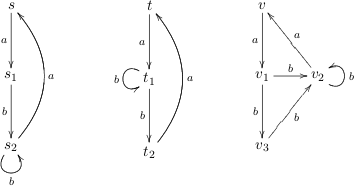
\includegraphics{qualitative-project/not-bisimilar-processes.png}
  \caption{Three not bisimilar processes}
  \label{fig:not-bisimilar-processes}
\end{figure}

\begin{verbatim}
Process s: RecX(a?.b?.RecY((b?.Y + a?.X)))
Process t: RecX(a?.RecY((b?.Y + b?.a?.X)))
Process v: RecX(a?.(b?.b?.RecY((b?.Y + a?.X)) + b?.RecY((b?.Y + a?.X))))

s isn't  bisimilar to t due to formula f= [a][b]<a>tt
s satisfy f: true
t satisfy f: false

s isn't  bisimilar to v due to formula f= [a]<b>[a]ff
s satisfy f: false
v satisfy f: true

t isn't  bisimilar to v due to formula f= [a]<b>[b]ff
t satisfy f: true
v satisfy f: false
\end{verbatim}

\subsection{Car-train crossing}

In this model we catch the situation of a cross of a road and a
rail. On both tracks a vehicle attempts to cross, a car and a train
respectively. In order to cross, a vehicle have to synchronize with a
``semaphore''.

We build the necessary \emph{CCS processes} in order to implement the
model and we proceed to verify the following properties:
\begin{itemize}
\item a train eventually cross, written in $\mu$-calculus using a min
  fix point:
  \begin{displaymath}
    \mu Z(\langle train\_cross\rangle tt \vee \langle Act
    \rangle Z)
  \end{displaymath}
\item it is no possible for the car and the train to cross
  simultaneously, written in $\mu$-calculus using a max fix point:
  \begin{displaymath}
    \nu Z(([train\_cross]ff \vee [car\_cross]ff) \wedge [Act]Z)
  \end{displaymath}
\item for each car $c$ that attempts to cross, $c$ eventually succeed,
  written in $\mu$-calculus using a mixture of min and max fix points:
  \begin{displaymath}
    \nu Z([car](\mu Y(\langle Act \rangle tt \wedge [-car\_cross]Y))
    \wedge  [-car]Z)
  \end{displaymath}
  It is interesting to note that the above formula does not use
  \emph{alternating fix points}, that is the variable $Z$ bounded by
  the out most $\nu$ does not appear in the context of the formula
  bounded by the innermost $\mu$. This is not the worst case for the
  $\mu$-calculus model checking (it is possible to write an equivalent
  \emph{aCTL} formula for the above one using the ``infinitely often''
  templates, while a formula with \emph{alternating fix points} has
  not an \emph{aCTL} equivalent).
\end{itemize}
Those properties are liveness, safety and fairness properties and
involve the solution of a min fixed point, a max fixed point and a
mixture of min and max fixed points respectively. We've written those
properties using our OCaml formula constructors and verified them with
the following results:
\begin{verbatim}
Process road: RecX(car?.up?.car_cross!.down!.X)
Process rail: RecY(train?.green?.train_cross!.red!.Y)
Process signal: RecZ((green!.red?.Z + up!.down?.Z))
Process crossing: (((RecX(car?.up?.car_cross!.down!.X) |
RecY(train?.green?.train_cross!.red!.Y)) | RecZ((green!.red?.Z +
up!.down?.Z))))\{green, red, up, down}
(((RecX(car?.up?.car_cross!.down!.X) |
RecY(train?.green?.train_cross!.red!.Y)) | RecZ((green!.red?.Z +
up!.down?.Z))))\{green, red, up, down}
Process crossing satisfy maxZ(([train_cross]ff or [car_cross]ff)
                                  and [Act]Z): true
Process crossing satisfy minZ(<train_cross>tt or <Act>Z): true
Process crossing satisfy maxZ([car](minY(<Act>tt and [-car_cross]Y))
                                  and  [-car]Z): true
\end{verbatim}

\subsection{$sat$ function code}
\label{subsec:sat-function-code}
In this section we report the code of the $sat$ function:
\lstset{language=Caml} 
\begin{lstlisting}
  let rec sat p = function
  | True -> true
  | Not f -> not (sat p f)
  | Or (f,g) -> (sat p f) || (sat p g)
  | And (f,g) -> (sat p f) && (sat p g)
  | Box (pred, f) ->
    let pred_matchers = List.find_all
      (fun (a, p') ->
	match a with
	| others -> pred a) (next p) in
    List.for_all (fun (a, p') -> sat p' f) pred_matchers
  | Diamond (pred, f) ->
    let pred_matchers = List.find_all
      (fun (a, p') ->
	match a with
	| others -> pred a) (next p) in
    List.exists (fun (a, p') -> sat p' f) pred_matchers
  | Min (var_name, seen_procs, f) ->
    if List.mem p seen_procs
    then false
    else sat p (unfold_formula var_name
                  (Min (var_name, (p::seen_procs), f)) f)
  | Max (var_name, seen_procs, f) ->
    if List.mem p seen_procs
    then true
    else sat p (unfold_formula var_name
                  (Max (var_name, (p::seen_procs), f)) f)
  | _ -> false;;
\end{lstlisting}

\bibliographystyle{alpha}
\bibliography{Her90,KNP12a,KNP11,QWP99,MuScSt1999,1324845}

\end{document} 
